\documentclass[11pt,twocolumn]{article}

\usepackage[utf8]{inputenc}
\usepackage[spanish]{babel}
\usepackage[T1]{fontenc}
\usepackage{amsmath}
\usepackage{amssymb}
\usepackage{graphicx}
\usepackage{float}
\usepackage{booktabs}
\usepackage[top=2.5cm,bottom=2.5cm,left=2cm,right=2cm]{geometry}
\usepackage{caption}
\usepackage{microtype}
\usepackage{parskip}
\usepackage{titlesec}
\usepackage{abstract}

\titleformat{\section}{\normalfont\bfseries\large}{\thesection.}{0.5em}{}
\titleformat{\subsection}{\normalfont\bfseries}{\thesubsection.}{0.5em}{}

\renewcommand{\abstractnamefont}{\normalfont\bfseries}
\renewcommand{\abstracttextfont}{\normalfont\small}

\title{\large\bfseries Magnetismo y Electromagnetismo: Visualizaci\'on de L\'ineas de Campo, Ley de Amp\`ere, Corrientes de Foucault e Inducci\'on Electromagn\'etica}

\author{
  Lina Cadavid Carrilo \quad Elida Ruiz Cantillo\\[4pt]
  {\small Universidad del Magdalena, Santa Marta}
}

\date{}

\begin{document}

\maketitle
\thispagestyle{plain}

\begin{abstract}
En esta pr\'actica de laboratorio se estudiaron experimentalmente cuatro fen\'omenos fundamentales del electromagnetismo: la visualizaci\'on de l\'ineas de campo magn\'etico, la verificaci\'on de la ley de Amp\`ere, las corrientes par\'asitas o de Foucault, y la inducci\'on electromagn\'etica aplicada a transformadores. En la primera mesa se visualizaron las l\'ineas de campo de un toroide, un solenoide y un im\'an cil\'indrico usando limadura de hierro. En la segunda mesa se verific\'o la ley de Amp\`ere con un sensor de campo magn\'etico sobre tres trayectorias cerradas alrededor de un aro con corriente, obteniendo $\oint \vec{B} \cdot d\vec{l} \approx \mu_0 N I_{\text{enc}}$ con error del 8,4\,\% cuando la trayectoria encierra la corriente y valores pr\'oximos a cero en los dem\'as casos. En la tercera mesa se estudi\'o el frenado magn\'etico por corrientes de Foucault en tres l\'aminas de aluminio con distintas geometr\'ias. En la cuarta mesa se verific\'o la relaci\'on del transformador $V_s/V_p = N_s/N_p$ y la dependencia de la fuerza electromotriz inducida con el n\'umero de espiras y la velocidad de variaci\'on del flujo.

\vspace{4pt}
\noindent\textbf{Abstract.}\; \textit{Four fundamental electromagnetic phenomena were studied experimentally. The first station visualized the magnetic field lines of a toroid, a solenoid, and a cylindrical magnet using iron filings. The second station verified Amp\`ere's law along three closed paths around a current-carrying loop, obtaining $\oint\vec{B}\cdot d\vec{l}\approx\mu_0 NI_{\rm enc}$ with an 8.4\,\% error when the path encloses the current, and near-zero values otherwise. The third station demonstrated eddy-current braking with three aluminum plates of different slot geometries. The fourth station confirmed $V_s/V_p = N_s/N_p$ and showed that the induced EMF depends on the number of turns and the rate of flux change.}
\end{abstract}

% ─────────────────────────────────────────────────────────────────────────────
\section{Introducci\'on}

El electromagnetismo constituye uno de los pilares fundamentales de la f\'isica cl\'asica, al describir la relaci\'on entre los fen\'omenos el\'ectricos y magn\'eticos que rigen el funcionamiento de una gran variedad de dispositivos tecnol\'ogicos modernos, desde generadores y motores el\'ectricos hasta transformadores y sistemas de freno magn\'etico.

En esta pr\'actica se desarrollaron cuatro experimentos que permiten explorar de forma visual y cuantitativa los conceptos clave del electromagnetismo: la geometr\'ia de las l\'ineas de campo, la ley de Amp\`ere, las corrientes de Foucault y la inducci\'on electromagn\'etica aplicada al transformador. La idea principal es que la f\'isica no se aprende s\'olo con ecuaciones: ver c\'omo la limadura de hierro dibuja las l\'ineas de campo de un solenoide, o c\'omo una l\'amina de aluminio frena en seco al pasar junto a un im\'an, proporciona una intuici\'on muy dif\'icil de transmitir \'unicamente con f\'ormulas.

La comprensi\'on de estos principios resulta adem\'as esencial en la formaci\'on de ingenieros, pues tiene aplicaci\'on directa en el dise\~no de sistemas el\'ectricos eficientes, la optimizaci\'on de transformadores y la implementaci\'on de tecnolog\'ias como la levitaci\'on magn\'etica y el frenado electromagn\'etico sin contacto mec\'anico.

% ─────────────────────────────────────────────────────────────────────────────
\section{Teor\'ia Relacionada}

\subsection*{L\'ineas de campo magn\'etico}

El campo magn\'etico $\vec{B}$ se representa mediante l\'ineas de campo: curvas cuya tangente en cada punto indica la direcci\'on del campo. A diferencia del campo el\'ectrico, estas l\'ineas son siempre cerradas, lo que se expresa con la ley de Gauss para el magnetismo:
\begin{equation}
  \oint_S \vec{B} \cdot d\vec{A} = 0,
\end{equation}
que nos dice que no existen monopolos magn\'eticos: todo im\'an tiene siempre un polo norte y un polo sur. En un solenoide de $n$ espiras por unidad de longitud con corriente $I$, el campo interior es uniforme:
\begin{equation}
  B = \mu_0 n I,
\end{equation}
con $\mu_0 = 4\pi\times10^{-7}\,\text{T\,m/A}$. En un toroide, el campo queda completamente confinado dentro del n\'ucleo y es nulo en el exterior. Las limaduras de hierro act\'uan como peque\~nos dipolos magn\'eticos que se alinean con la direcci\'on del campo, permitiendo visualizar sus l\'ineas de fuerza.

\subsection*{Ley de Amp\`ere}

La ley de Amp\`ere establece que la integral del campo magn\'etico a lo largo de cualquier camino cerrado es proporcional a la corriente que ese camino encierra:
\begin{equation}
  \oint_C \vec{B} \cdot d\vec{l} = \mu_0 \sum I_{\text{enc}}.
\end{equation}
Lo m\'as importante de esta ley es que no depende de la forma del camino, sino de si ese camino encierra o no al conductor con corriente. Si el camino no pasa alrededor de ninguna corriente, la integral da cero sin importar c\'omo sea el trayecto. Aunque la ley de Amp\`ere original s\'olo es v\'alida para situaciones de magnetost\'atica, fue corregida por Maxwell para aplicarse tambi\'en en campos el\'ectricos no estacionarios.

\subsection*{Corrientes de Foucault}

Las corrientes par\'asitas o de Foucault son corrientes el\'ectricas inducidas en materiales conductores cuando est\'an sometidos a una variaci\'on del flujo magn\'etico. Por la ley de Lenz, estas corrientes se oponen al movimiento, generando una fuerza de frenado. Qu\'e tan intensas sean depende de la geometr\'ia del conductor: en una placa s\'olida los electrones pueden circular en lazos grandes, generando corrientes intensas y mucho frenado; si se le hacen ranuras, esos caminos se interrumpen y el frenado disminuye. Este principio justifica que los n\'ucleos de los transformadores se fabriquen con l\'aminas delgadas apiladas separadas por capas aislantes.

\subsection*{Inducci\'on y transformador}

La ley de Faraday establece que una fuerza electromotriz (fem) se induce en una bobina cuando el flujo magn\'etico que la atraviesa var\'ia:
\begin{equation}
  \mathcal{E} = -N\frac{d\Phi_B}{dt},
\end{equation}
donde $N$ es el n\'umero de espiras. El signo negativo corresponde a la ley de Lenz: la corriente inducida siempre se opone al cambio que la produce. A m\'as espiras, mayor fem; y a mayor velocidad de cambio del flujo, tambi\'en mayor fem. El transformador usa este principio acoplando dos bobinas mediante un n\'ucleo de hierro; la relaci\'on entre los voltajes es:
\begin{equation}
  \frac{V_s}{V_p} = \frac{N_s}{N_p},
\end{equation}
donde los sub\'indices $p$ y $s$ indican el devanado primario y secundario respectivamente.

% ─────────────────────────────────────────────────────────────────────────────
\section{Montaje y Procedimiento}

\subsection*{Mesa 1: Visualizaci\'on de l\'ineas de campo}

Se conectaron un toroide y un solenoide de alambre de cobre a una fuente de corriente directa de aproximadamente 2,9\,V. Se distribuy\'o limadura de hierro alrededor de cada uno y, al encender la fuente y dar peque\~nos golpes al soporte, las part\'iculas se alinearon con las l\'ineas de campo mostrando claramente su geometr\'ia. Tambi\'en se dispon\'ia de un im\'an cil\'indrico dentro de una c\'apsula acr\'ilica transparente rellena de limadura de hierro, que permit\'ia visualizar las l\'ineas de campo en tres dimensiones.

\begin{figure}[H]
  \centering
  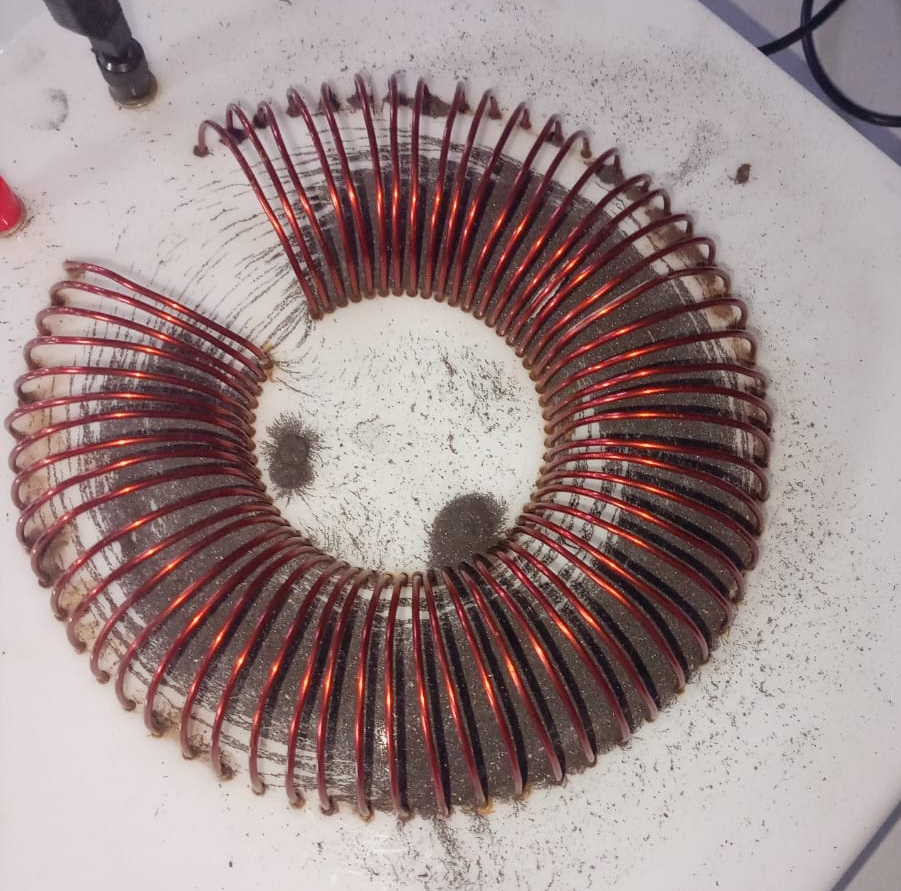
\includegraphics[width=\linewidth]{toroide.jpg}
  \caption{Toroide con limadura de hierro. Las l\'ineas de campo quedan completamente confinadas dentro del n\'ucleo toroidal, con flujo nulo en el exterior.}
  \label{fig:toroide}
\end{figure}

\begin{figure}[H]
  \centering
  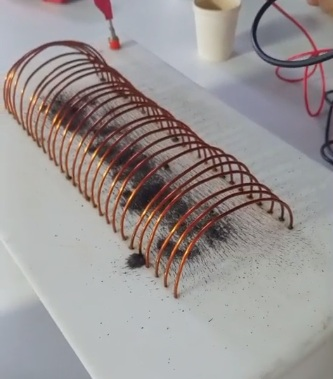
\includegraphics[width=\linewidth]{solenoide.jpg}
  \caption{Solenoide con limadura de hierro. Las l\'ineas emergen por un extremo y se cierran por el otro, igual que en un im\'an de barra.}
  \label{fig:solenoide}
\end{figure}

\subsection*{Mesa 2: Verificaci\'on de la ley de Amp\`ere}

Se utiliz\'o el aparato PASCO Ampere's Law (EM-6720): una plataforma con un aro conductor circular con corriente conocida, y un carro con sensor inal\'ambrico de campo magn\'etico que se desplaza manualmente. El software PASCO Capstone registra $B_x$ en funci\'on de la posici\'on y calcula la integral $\oint\vec{B}\cdot d\vec{l}$ como el \'area bajo esa curva.

Con $I \approx 0{,}815\,\text{A}$ y $\mu_0 NI \approx 5{,}12\,\text{G\,m}$ se realizaron tres recorridos cerrados:
\begin{itemize}
  \item \textbf{Recorrido 1:} el carro pasa por el centro del aro, enlazando la corriente.
  \item \textbf{Recorrido 2:} el carro rodea el exterior del aro completo sin pasar por el centro.
  \item \textbf{Recorrido 3:} el carro recorre solo un lado del aro.
\end{itemize}

En uno de los recorridos el sensor se desplaz\'o por dentro del aro y el sistema arroj\'o una gr\'afica con forma de campana de Gauss, con el punto m\'as alto cuando el sensor pasaba por el centro del aro.

\subsection*{Mesa 3: Corrientes de Foucault}

Se colgaron tres l\'aminas planas de aluminio de una barra horizontal para que oscilaran como p\'endulos. Justo debajo, dos imanes permanentes enfrentados generaban un campo magn\'etico concentrado y estable, de modo que las l\'aminas pasaban entre sus polos al balancearse. Las tres l\'aminas presentaban geometr\'ias distintas:
\begin{enumerate}
  \item \textbf{L\'amina s\'olida:} sin cortes, superficie continua.
  \item \textbf{L\'amina con orificios cerrados:} recortes rectangulares que no llegan a ning\'un borde.
  \item \textbf{L\'amina tipo peine:} ranuras finas y densas abiertas en el borde inferior, formando \textit{dientes} separados en la parte baja pero unidos por un puente s\'olido en la parte superior.
\end{enumerate}
Cada ensayo se repiti\'o varias veces bajo las mismas condiciones para garantizar la confiabilidad de las observaciones.

\subsection*{Mesa 4: Transformador e inducci\'on con im\'an}

Se utilizaron bobinas intercambiables Frederiksen (200, 400, 800, 1600 y 3200 espiras) con un n\'ucleo de hierro en U y una pieza de cierre (yugo). La bobina primaria se conect\'o a una fuente de corriente alterna de 5\,V y la secundaria a un mult\'imetro en modo voltaje AC. Se probaron diversas combinaciones de bobinas midiendo el voltaje en el secundario.

\begin{figure}[H]
  \centering
  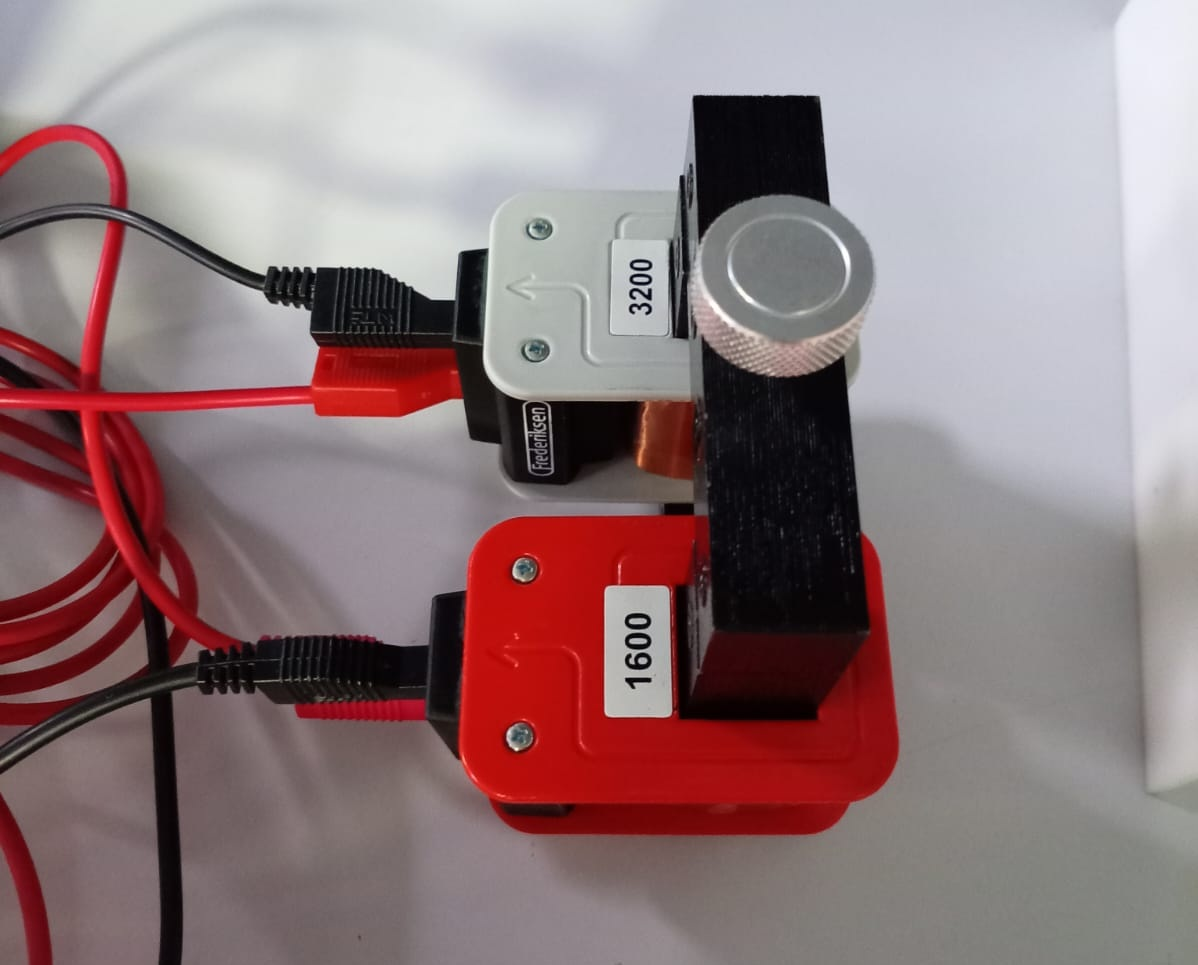
\includegraphics[width=\linewidth]{bobinas.jpg}
  \caption{Bobinas Frederiksen sobre el n\'ucleo de hierro en U utilizadas en el experimento del transformador.}
  \label{fig:bobinas}
\end{figure}

Posteriormente se desconect\'o el n\'ucleo, se conect\'o una sola bobina al volt\'imetro y se pas\'o un im\'an (primero delgado, luego grande) a trav\'es de ella varias veces, registrando la fem m\'axima para bobinas de 200, 400 y 3200 espiras.

\begin{figure}[H]
  \centering
  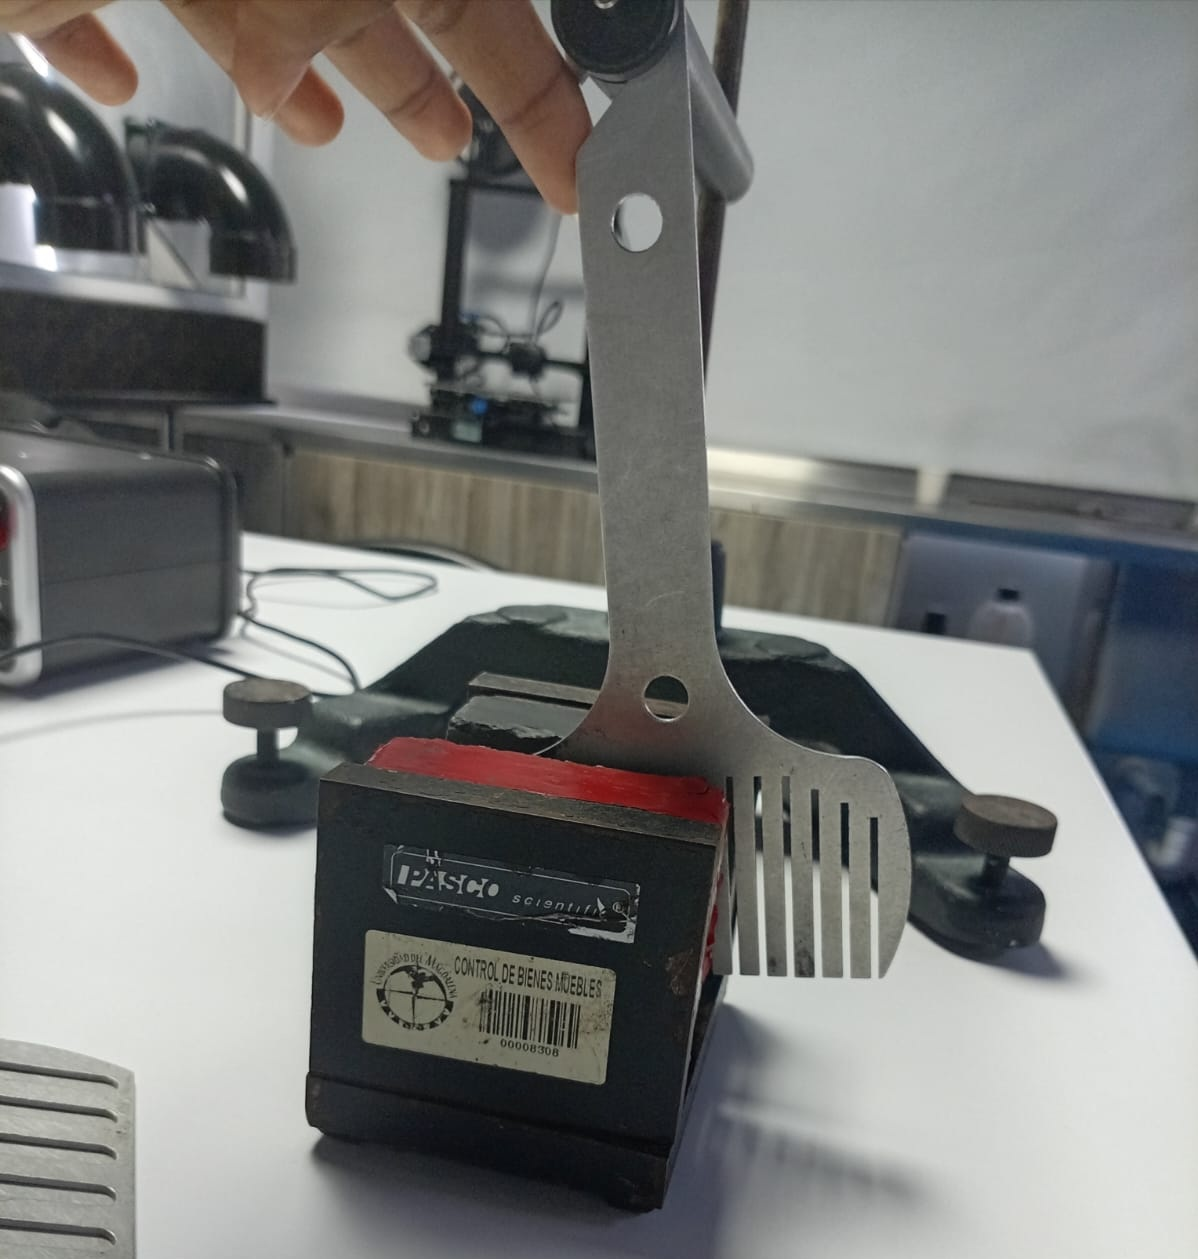
\includegraphics[width=\linewidth]{barra.jpg}
  \caption{Im\'an de barra utilizado en el experimento de inducci\'on para generar fem en las bobinas al desplazarse a trav\'es de ellas.}
  \label{fig:barra}
\end{figure}

% ─────────────────────────────────────────────────────────────────────────────
\section{Resultados}

\subsection*{Mesa 1}

La limadura se aline\'o de inmediato al encender la fuente. En el toroide (Fig.~\ref{fig:toroide}), las l\'ineas quedaron completamente dentro del n\'ucleo. En el solenoide (Fig.~\ref{fig:solenoide}) se formaron l\'ineas axiales densas que emerg\'ian por los extremos. El im\'an cil\'indrico en la c\'apsula 3D mostr\'o el patr\'on dipolar cl\'asico: l\'ineas saliendo de un polo y cerr\'andose en el otro.

\subsection*{Mesa 2 -- Ley de Amp\`ere}

Los resultados de cada recorrido se muestran en la Tabla~\ref{tab:ampere}.

\begin{table}[H]
  \centering
  \caption{Integral de l\'inea en los tres recorridos. $I = 0{,}815\,\text{A}$, $\mu_0 NI = 5{,}12\,\text{G\,m}$.}
  \label{tab:ampere}
  \begin{tabular}{lcc}
    \toprule
    Trayectoria & \'{A}rea (G\,m) & Enlaza $I$? \\
    \midrule
    Por el centro   & 5,55  & S\'i \\
    Rodea exterior  & 0,933 & No  \\
    Solo un lado    & 0,263 & No  \\
    \bottomrule
  \end{tabular}
\end{table}

\subsection*{Mesa 3 -- Corrientes de Foucault}

Al soltar las tres l\'aminas con la misma amplitud inicial:
\begin{itemize}
  \item \textbf{L\'amina s\'olida:} se fren\'o notoriamente al pasar entre los imanes, deteni\'endose casi por completo.
  \item \textbf{L\'amina con orificios cerrados:} present\'o un frenado similar al de la l\'amina s\'olida.
  \item \textbf{L\'amina tipo peine:} se detuvo de forma muy abrupta; el puente s\'olido superior permite lazos de corriente de gran \'area.
\end{itemize}

\subsection*{Mesa 4 -- Transformador e inducci\'on}

\textbf{Transformador:} La Tabla~\ref{tab:transformador} compara los voltajes te\'oricos y medidos para las combinaciones realizadas con la fuente a 5\,V.

\begin{table}[H]
  \centering
  \caption{Resultados del transformador ($V_p = 5\,\text{V}$ AC).}
  \label{tab:transformador}
  \begin{tabular}{ccccc}
    \toprule
    $N_p$ & $N_s$ & $V_s^{\text{te\'or.}}$ & $V_s^{\text{med.}}$ & Efic. \\
    \midrule
    1600 & 3200 & 10,0 V & 8,2 V  & 82\,\% \\
    1600 &  400 &  1,3 V & 1,0 V  & 80\,\% \\
     200 & 3200 & 80,0 V & 31,3 V & 39\,\% \\
     200 & 1600 & 40,0 V & 35,4 V & 89\,\% \\
    \bottomrule
  \end{tabular}
\end{table}

Adicionalmente se realizaron pruebas con otras combinaciones: para $N_p=200$ y $N_s=800$ se obtuvo $V_s=14{,}1\,\text{V}$; para $N_p=200$ y $N_s=3200$ el voltaje alcanz\'o aproximadamente 71\,V.

\textbf{Inducci\'on con im\'an:} La Tabla~\ref{tab:induccion} resume los rangos de fem medidos.

\begin{table}[H]
  \centering
  \caption{Fem inducida al mover los imanes (los valores dependen de la velocidad de paso).}
  \label{tab:induccion}
  \begin{tabular}{lcc}
    \toprule
    Bobina & Im\'an delgado & Im\'an grande \\
    \midrule
    200 espiras  & 0 -- 29,7 mV & 0 -- 3,4 mV \\
    400 espiras  & 0 -- 30 mV   & 1 -- 7,4 mV \\
    3200 espiras & 0 -- 4,8 V   & 0 -- 83 mV  \\
    \bottomrule
  \end{tabular}
\end{table}

% ─────────────────────────────────────────────────────────────────────────────
\section{An\'alisis}

\subsection*{Mesa 1}

Los resultados confirman lo que predice la teor\'ia. En el toroide, el campo queda totalmente encerrado en su interior, lo que explica por qu\'e esa geometr\'ia se utiliza en electr\'onica cuando se quiere evitar que el campo magn\'etico interfiera con otros componentes. En el solenoide, las l\'ineas en el interior son paralelas y uniformes y se cierran por los extremos, de modo id\'entico a un im\'an de barra, lo que justifica el nombre de \textit{electroim\'an} cuando se incorpora un n\'ucleo de hierro. El im\'an cil\'indrico en la c\'apsula 3D deja claro que los diagramas de campo en papel son \'unicamente un corte de algo que ocurre en todas las direcciones del espacio.

\subsection*{Mesa 2 -- Ley de Amp\`ere}

Para el Recorrido 1 (por el centro), el \'area medida fue $5{,}55\,\text{G\,m}$ frente al valor te\'orico $\mu_0 NI = 5{,}12\,\text{G\,m}$, lo que da un error relativo de:
\begin{equation}
  \varepsilon_1 = \frac{|5{,}55 - 5{,}12|}{5{,}12}\times 100\,\% \approx 8{,}4\,\%.
\end{equation}
Este error, razonablemente peque\~no, se debe principalmente a que el carro no traza un camino perfectamente cerrado, a peque\~nas vibraciones del sensor durante el desplazamiento y a posibles interferencias de otros equipos en el laboratorio.

Para los Recorridos 2 y 3, que no enlazan la corriente, los valores obtenidos ($0{,}933\,\text{G\,m}$ y $0{,}263\,\text{G\,m}$) son m\'as de diez veces menores que el del Recorrido~1. Esta diferencia de magnitud confirma el principio central de la ley de Amp\`ere: lo que determina el valor de la integral no es la forma del camino, sino si ese camino encierra o no la corriente. Cuando el camino pasa por el centro del aro y enlaza la corriente, la integral es aproximadamente $\mu_0 NI$; cuando no la encierra, la integral es pr\'acticamente cero.

\subsection*{Mesa 3 -- Corrientes de Foucault}

Lo que determina cu\'anto se frena cada l\'amina es si existen caminos cerrados disponibles para que las corrientes puedan circular. La l\'amina s\'olida no tiene ninguna interrupci\'on, as\'i que los electrones pueden describir lazos grandes que encierran mucho flujo; por la ley de Lenz, eso genera corrientes que frenan la l\'amina con mucha fuerza.

La l\'amina tipo peine es el caso m\'as interesante. Tiene ranuras abiertas en el borde inferior, pero la parte superior es un puente s\'olido continuo que conecta todos los dientes. Cuando la l\'amina pasa entre los imanes, las corrientes circulan siguiendo un recorrido en forma de U invertida: suben por un diente, cruzan el puente superior y bajan por el diente adyacente. Este lazo encierra pr\'acticamente la misma \'area que en una l\'amina s\'olida, de modo que la fem inducida es igualmente grande y el frenado es igualmente intenso.

La clave est\'a en que no basta con hacer cortes en un conductor para eliminar las corrientes de Foucault. Los cortes deben romper completamente todos los lazos posibles; si queda un puente s\'olido conectando las tiras, la corriente sigue encontrando camino. Este es exactamente el motivo por el que los n\'ucleos de los transformadores se fabrican con l\'aminas delgadas separadas por capas aislantes.

\subsection*{Mesa 4 -- Transformador e inducci\'on}

\textbf{Transformador:} Para primarios de 1600 espiras la eficiencia fue del 80--82\,\%, coherente con las p\'erdidas normales de un transformador de laboratorio: resistencia del alambre, hist\'eresis en el n\'ucleo y flujo que no llega al secundario. El caso m\'as llamativo es el primario de 200 espiras con secundario de 3200 (fila~3 de la Tabla~\ref{tab:transformador}): se midieron $31{,}3\,\text{V}$ en lugar de los 80\,V te\'oricos (apenas un 39\,\% de eficiencia). Esto ocurre porque con tan pocas espiras en el primario, su inductancia es muy baja (la inductancia crece con $N_p^2$, por lo que pasar de 1600 a 200 espiras la reduce 64 veces), haciendo que gran parte de la energ\'ia se disipe en calor en lugar de transferirse al secundario.

\textbf{Inducci\'on con im\'an:} Los datos de la Tabla~\ref{tab:induccion} muestran que la fem crece con el n\'umero de espiras, en l\'inea con la ley de Faraday. Para el im\'an grande:
\begin{equation}
  \frac{\mathcal{E}_{400}}{\mathcal{E}_{200}} = \frac{7{,}4}{3{,}4} \approx 2{,}2 \approx \frac{400}{200} = 2 \quad (\checkmark).
\end{equation}
La raz\'on $\mathcal{E}_{3200}/\mathcal{E}_{200}\approx 24$ es algo mayor que el factor te\'orico 16, lo que se explica porque ese ensayo se realiz\'o con mayor velocidad de paso del im\'an, amplificando la fem. En conjunto, los resultados verifican cuantitativamente que $\mathcal{E}\propto N$ y que la velocidad del im\'an tiene un efecto directo sobre la magnitud de la fem inducida.

% ─────────────────────────────────────────────────────────────────────────────
\section{Conclusiones}

Los cuatro experimentos permitieron verificar de forma directa los principios fundamentales del electromagnetismo cl\'asico.

La visualizaci\'on con limadura de hierro demostr\'o que las l\'ineas de campo son lazos cerrados cuya geometr\'ia depende de la configuraci\'on del conductor o im\'an: el toroide las confina completamente, el solenoide las proyecta axialmente y el im\'an cil\'indrico las distribuye en forma dipolar en tres dimensiones.

La verificaci\'on de la ley de Amp\`ere confirm\'o su car\'acter topol\'ogico: cuando el camino encierra la corriente, la integral vale $\approx\mu_0 NI$ (error del 8,4\,\%); cuando no la encierra, el resultado es pr\'acticamente cero, independientemente de la forma del trayecto.

En las corrientes de Foucault se comprob\'o que la geometr\'ia de las ranuras es determinante. La l\'amina tipo peine se fren\'o de manera muy abrupta porque su puente s\'olido superior permite que las corrientes formen lazos de gran \'area entre los dientes. Esto muestra que los cortes solo reducen el frenado si interrumpen completamente todos los lazos de corriente posibles, principio que justifica el uso de n\'ucleos laminados en transformadores y m\'aquinas el\'ectricas.

Finalmente, el transformador confirm\'o la relaci\'on $V_s/V_p = N_s/N_p$ con eficiencias del 80--89\,\% para primarios de 1600 espiras, pero con apenas el 39\,\% para el primario de 200 espiras, evidenciando que la inductancia del primario es clave para un buen desempe\~no. El experimento de inducci\'on con im\'an verific\'o que $\mathcal{E}\propto N$ y que la velocidad del im\'an afecta directamente la fem inducida.

% ─────────────────────────────────────────────────────────────────────────────
\section*{Referencias}

\begin{enumerate}\setlength\itemsep{2pt}
  \item D.\,J.~Griffiths, \textit{Introduction to Electrodynamics}, 4.\textsuperscript{a}\,ed., Cambridge University Press (2017).
  \item P.\,A.~Tipler y G.~Mosca, \textit{F\'isica para la Ciencia y la Tecnolog\'ia}, vol.\,2, 6.\textsuperscript{a}\,ed., Rever\'e (2010).
  \item H.\,D.~Young y R.\,A.~Freedman, \textit{Sears-Zemansky F\'isica Universitaria}, vol.\,2, 14.\textsuperscript{a}\,ed., Pearson (2018).
  \item S.\,J.~Chapman, \textit{Electric Machinery Fundamentals}, 5.\textsuperscript{a}\,ed., McGraw-Hill Education (2012).
  \item D.~Halliday, R.~Resnick y J.~Walker, \textit{Fundamentals of Physics}, 10.\textsuperscript{a}\,ed., Wiley (2014).
  \item R.\,A.~Serway y J.\,W.~Jewett, \textit{Physics for Scientists and Engineers}, 10.\textsuperscript{a}\,ed., Cengage Learning (2018).
  \item PASCO Scientific, \textit{Ampere's Law Apparatus EM-6720 Instruction Manual}, PASCO (2019).
  \item Frederiksen, \textit{Transformer Coils 2855.00 User Guide}, Frederiksen (2015).
\end{enumerate}

\end{document}
